\newcommand{\mypapersize}{A4}
%% e.g., "A4", "letter", "legal", "executive", ...
%% The size of the paper of the resulting PDF file.

\newcommand{\mylaterality}{oneside}
%% "oneside" or "twoside"
%% Either you are creating a document which is printed on both, left pages
%% and right pages (twoside) or you create a document which is printed
%% on right pages only (oneside).

\newcommand{\mydraft}{false}
%% "true" or "false"
%% Use draft mode? If true, included graphics are replaced by empty
%% rectangles (of same size) and overfull boxes (in margin space) are
%% marked with black box (-> easy to spot!)

\newcommand{\myparskip}{no}
\setlength{\parindent}{2em}
%% e.g., "no", "full", "half", ...
%% How to separate paragraphs: indention ("no") or spacing ("half",
%% "full", ...).

\newcommand{\myBCOR}{0mm}
%% Inner binding correction. This value depends on the method which is
%% being used to bind your printed result. Some techniques do not
%% require a binding correction at all ("0mm"), other require for
%% example "5mm". Refer to KOMA script documentation for a detailed
%% explanation what a binding correction is and how to measure it.

\newcommand{\myfontsize}{12pt}
%% e.g., 10pt, 11pt, 12pt
%% The font size of the main text in pt (points).

\newcommand{\mylinespread}{1.0}
%% e.g., 1.0, 1.5, 2.0
%% Line spacing in %/100. For example 1.5 means 150% of the usual line
%% spacing. Please use with caution: 100% ("1.0") is fine because the
%% font was designed for it.

\newcommand{\mylanguage}{american}
%% "english,ngerman", "ngerman,english", ...
%% NOTE: The *last* language is the active one!
%% See babel documentation for further details.

%% BibLaTeX-settings: (see biblatex reference for further description)
\newcommand{\mybiblatexstyle}{apa}
%% e.g., "alphabetic", "authoryear", ...
%% The biblatex style which is being used for referencing. See
%% biblatex documentation for further details and more values.

\newcommand{\mybiblatexdashed}{false}  %% "true" or "false"
%% If true: replace recurring reference authors with a dash.

\newcommand{\mybiblatexbackref}{true}  %% "true" or "false"
%% If true: create backward links from reference to citations.

\newcommand{\mybiblatexfile}{references-biblatex.bib}
%% Name of the biblatex file that holds the references.

\newcommand{\mydispositioncolor}{0,0,0}
%% e.g., "30,103,182" (blue/turquois), "0,0,0" (black), ...

\newcommand{\mycolorlinks}{true}  %% "true" or "false"
%% Enables or disables colored links (hyperref package).

\newcommand{\mytitlepage}{template/title_Thesis_TU_Graz}

%% Load main settings for document preamble:
\input{template/preamble}%% DO NOT REMOVE THIS LINE!


\setboolean{english_affidavit}{true}  %% "true" or "false"

%% ========================================================================
%%%% Document metadata
%% ========================================================================

\newcommand{\myauthor}{Fabian Santer}
\newcommand{\myauthorwithexistingtitles}{\myauthor{}}
\newcommand{\mytitle}{Real-time Anomaly Detection in Time Series Data}
\newcommand{\mysubject}{SUBJECT}
\newcommand{\mykeywords}{KEYWORDS}

\newcommand{\myworktitle}{Bachelor's Thesis}
\newcommand{\mygrade}{Bachelor of Science}
\newcommand{\mystudy}{}
\newcommand{\mydegreeprogramme}{Bachelor's degree programme : Software Engineering and Management \mystudy}
\newcommand{\mydegreeprogrammegerman}{Masterstudium: \mystudy}
\newcommand{\myuniversity}{Graz University of Technology}
\newcommand{\myuniversitygerman}{Technische Universität Graz}
\newcommand{\myinstitute}{Institute of Visual Computing}
\newcommand{\myinstitutehead}{Univ.-Prof. Dipl.-Ing. Dr.techn. Thomas Pock}
\newcommand{\mysupervisor}{Dipl.-Math. Dr.techn. Ullrich Torsten}
\newcommand{\mycosupervisors}{}
\newcommand{\myevaluator}{Prof.~Some Genius}
\newcommand{\myhomestreet}{Aufkirchen 37}
\newcommand{\myhometown}{Toblach}
\newcommand{\myhomepostalnumber}{39034}
\newcommand{\mysubmissionmonth}{month}
\newcommand{\mysubmissionyear}{year}
\newcommand{\mysubmissiontown}{Graz}

\newcommand{\myid}{12230815}
\newcommand{\mylecture}{LECTURE}


%% ========================================================================
%%%% MISC command definitions
%% ========================================================================
\input{template/mycommands}

%% ========================================================================
%%%% Typographic settings
%% ========================================================================
\input{template/typographic_settings}


%% ========================================================================
%%%% MISC usepackages
%% ========================================================================

\usepackage{soul}
\usepackage{booktabs}
\usepackage{amsmath}
\usepackage{placeins}
\usepackage{geometry}
\usepackage{pdfpages}
\usepackage{verbatim}
\usepackage{tikz}
\usetikzlibrary{arrows,calc,positioning,fit}
\usepackage{float}

% Code listing configuration
\usepackage{color}
\usepackage{listings}

% Define color palette
\definecolor{javared}{rgb}{0.6,0,0}           % for strings
\definecolor{javagreen}{rgb}{0.25,0.5,0.35}   % comments
\definecolor{javapurple}{rgb}{0.5,0,0.35}    % keywords
\definecolor{javadocblue}{rgb}{0.25,0.35,0.75}% javadoc/docstrings

\lstset{
  inputpath={},                               % Overrides template default inputpath
  language=C,
  escapeinside={//(*}{*)},
  captionpos=t,
  numbers=left,
  stepnumber=5,
  numbersep=5pt,
  numberstyle=\scriptsize\color{black},
  showspaces=false,
  showtabs=false,
  breaklines=true,
  showstringspaces=false,
  breakatwhitespace=true,
  basicstyle=\fontsize{7.5}{7.5}\selectfont\ttfamily,
  keywordstyle=\color{javapurple}\bfseries,
  stringstyle=\color{javared},
  commentstyle=\color{javagreen},
  morecomment=[s][\color{javadocblue}]{/**}{*/}
}

\geometry{a4paper, portrait, tmargin=1.5in, bmargin=1.5in, outer=1.5in}

%% ========================================================================
%%%% MISC self-defined commands and settings
%% ========================================================================

\newcommand{\myLaT}{\LaTeX{}@TUG\xspace}

\hyphenation{ex-am-ple hy-phen-ate}

\input{template/pdf_settings}  %% should be *last* definitions in preamble!

%% ========================================================================
%%%% begin{document}
%% ========================================================================
\begin{document}

\frontmatter                    %% KOMA: roman page numbers and such

\input{\mytitlepage}

\input{template/declaration_TU_Graz}

\chapter*{Abstract}\label{cha:abstract}
This is a placeholder for the abstract. It summarizes the whole thesis
to give a very short overview. Usually, this the abstract is written
when the whole thesis text is finished.

Aufgaben: Max. 1 Seite

Eine der Funktionen des Abstract deiner Bachelorarbeit ist, dass der Leser einschätzen kann, ob der Inhalt deiner Arbeit für ihn interessant ist. Du beantwortest im Abstract vier Fragen:
Was ist das Thema?
Was wurde untersucht?
Was ist das Ergebnis?
Was bedeuten deine Ergebnisse?\\

The thesis investigates the combination of three individual concepts: time delay embedding, principle component analysis and sliding window techniques. The aim is to transform an offline algorithm for vibration signal analysis into an efficient real-time streaming version. The overall goal is to develop an incremental computation approach for principle component analysis that reuses previously calculated values rather than calculating everything from scratch over and over again, thereby reducing computational overhead. Building on the work of \cite{rakuschek2025visual}, the original offline algorithm is extended into an incremental, online implementation which is able to process continuous data streams and use the incremental principle component analysis on this data.
The resulting product, written in C, is designed for straightforward integration into existing systems that require principle component analyis on streaming data.

\newpage\null\thispagestyle{empty}\newpage



\tableofcontents

\listoffigures

\listoftables

\mainmatter                     %% KOMA: marks main part using arabic page numbers

\chapter{Introduction}
Industrial facilities are increasingly equipped with vibration sensors that generate thousands of measurements per seconds. During a single test run a electrical motor can easily produce thousands of data points per minutes as demonstrated by the dataset used in this thesis. This amount of data is not meant to be stored but monitored in real time so that even an non expert in the domain can detect faults early before a complete machine failure. While there are is a solution to this issue namely principal component analysis, which is the main topic of this thesis, still rely on static full available datasets and is (still) not optimized for streaming data and real time anomaly detection. \\\\
The early detection of mechanical anomalies, such as unnatural vibration development, is a central piece of predictive maintenance and therefore a valuable asset to industry. Unplanned downtime or intensive maintenance are significantly costs to consider while easy monitoring can reduce faults and extend the lifespan of an machine. From a scientific perspective principal component analysis is relevant because its combination with time delay embedding as proposed by \textcite{rakuschek2025visual} produces a powerful visually interpretable "fingerprint" of vibration signals, yet only a offline method was described. Taking this method and transferring it into a streaming context comes along with some difficulties such as how to update the algorithm to eliminate computational bottlenecks and to adapt each part of the algorithm to the new streaming approach. When this is achieved it enables the transition from an academic proof of concept to an deployable application.\\ \\
The current state of research are two separate concepts to be investigated. On one hand \textcite{rakuschek2025visual} combines time delay embeddings and principal component analysis to reveal periodic behavior of vibration signals but under the restriction that the full signal history has to be present and that the covariance matrix and its eignedecomposition has to be recomputed from scratch each time a new data point arrives. This makes the offline inefficient and not suitable for high interval streaming data. Another concept investigated in this thesis is the incremental principal component analysis approach by \textcite{Incremental_PCA} along with subspace tracking from \textcite{Oja1982SimplifiedNM} which is a tool for iteratively approximating eigenvectors without calculating the full eignedecomposition solving one of the many computational bottlenecks discussed in this thesis. However these two concepts have not yet been combined with time delay embedding and sliding window mechanism into a single casted real time capable streaming application.\\ \\
The central research question of this thesis is to explore if an incremental, streaming version if the algorithm proposed by \textcite{rakuschek2025visual} keep the diagnostic quality of the of the offline implementation while reducing computational cost with incremental updates of the covariance matrix and eigenvectors. Additionally this thesis investigates how the principal component analysis parameters embedding dimension, time delay and window size influence the quality of the resulting fingerprint plot. \\ \\
To solve this challenge a platform independent library written in C/C++ is developed, which is oriented on the offline algorithm with the improvement that running statistics (mean,covariance matrix etc.) as well as the dominant eigenvectors via subspace iteration are updated incrementally instead of recomputing them from scratch with each incoming data point. The thesis is structured as follows: Chapter 2 investigates the theoretical foundations of time delay embedding, principal component analysis and sliding window techniques and explains in detail how the original implementation is structured. Chapter 3 justifies the selection of the used tech stack and validates the used datasets. Chapter 4 explains in detail the concrete implementation of the combination of the three individual concepts and reinforces that with mathematical formulas and code snippets. Chapter 5 compares the concrete implementation against a reference computation and evaluates the resulting fingerprint plots on real vibration datasets with different parameters applied on. Finally chapter 6 and 7 summarize the findings and provide an outlook on future possible applications.
% Spellchecking done with grammarly
\chapter{Background and Related Work}
As mentioned in the introduction, the high computational cost of principal component analysis introduces a significant challenge for real-time anomaly detection, especially as the volume of data grows really large. To address this limitation, \parencite[p.~1]{rakuschek2025visual} proposed combining time delay embedding (TDE) with principal component analysis (PCA). His final implementation generates visual plots from vibration data that resemble human fingerprints. This chapter explains the theoretical foundations of principal component analysis and time delay embedding in detail, identifies key computational bottlenecks, and reviews the original offline implementation of the algorithm.

% Spellchecking done with grammarly
\section{Baseline Methodology}
The purpose of the underlying paper was to create an algorithm which solves the issue of plotting vibration data on a line graph where the observer can't distinguish between noise and the actual vibrations. The overall goal was to: further enhance and complement the visual inspection in the time
domain, enabling users to quickly gain an overview of different
vibration profiles within the signal or to detect periodicity within
noise. (\cite{rakuschek2025visual} p.1). In the background this was done by using  time delay embeddings, which is a method that takes the time series data and transforms it into a point cloud which can than be projected onto a 2D plane. Another really important aspect of the algorithm which is to be transformed is the use of principal component analysis. It is a dimensionality reduction technique that helps reduce the number of features in a dataset while keeping the most important information. As stated by \textcite{KarlPearson}, principal component analysis simplifies complex datasets by transforming correlated features into a smaller set of uncorrelated components. When the two algorithms are applied on a harmonic oscillation the result is a ellipsoid and as more noise is added its really hard to distinguished between noise or the hidden signal. However, applying time delay embedding with appropriate window sizes effectively reveals the underlying vibration signal.

% Spellchecking done with grammarly
{\section{Concepts}}

In the following paragraphs the offline  algorithm by \cite{rakuschek2025visual} is explained in more detail. Additionally the  main underlying mathematical methods, namely PCA,TDE and sliding Windows are discussed. Finally an overview over the related work is provided.

\subsection{Time delay Embeddings}
Time Delay Embedding (TDE) creates a multidimensional geometrical object from a single time series signal. Given a scalar signal $x(t)$, where $x(t) \in {R}$ represents any measurement at time $t$, standard one dimensional analysis often fails to reveal underlying structural properties. In contrast, the embedding transforms the temporal signal to a multidimensional space, revealing underlying attractors, trajectories, and regime changes. This turns the dynamic temporal problem into a geometric problem which is significantly easier to solve. Under optimal operating conditions, the signal traces clear, predictable geometric shapes (such as ellipsoids, straight lines or circles), making normal behavior easy to distinguish from anomalies. The embedded state vector $X(t)$ is constructed as:
$$X(t) = [x(t), x(t - \tau), x(t - 2\tau), \dots, x(t - (d - 1)\tau)]$$
where $x(t)$ represents the continuous signal at time $t$, $d$ denotes the embedding dimension, and $\tau$ is the time delay. 
For discrete time series data $x = [x_1, x_2, x_3, \dots, x_N]$, choosing $d = 3$ and $\tau = 1$ transforms the sequence $[x_1, x_2, x_3, x_4, x_5]$ into the following set of 3D points:
$$[x_1, x_2, x_3], \quad [x_2, x_3, x_4], \quad [x_3, x_4, x_5]$$
The embedding dimension $d$ defines how many past samples are used to reconstruct the state. If the parameter $d$ is chosen too small, the dynamics are not fully shown; if chosen too large, the noise is amplified. The delay $\tau$ defines the spacing between the samples. \\
Periodic machine vibrations naturally map to elliptical structures, this geometric behavior is the result of plotting a harmonic signals $x(t)$ against its time delayed counterpart $x(t - \tau)$ which forms a two dimensional phase plot, where periodic oscillations trace a closed elliptical trajectory. In contrast random uncorrelated noise forms a scattered cloud.
As stated by \textcite[p.~4]{rakuschek2025visual}, TDEs serve as an effective fingerprinting technique for vibration signals, enabling clear visual identification of changes in vibration profiles and underlying periodicity.
\subsection{Principal Component Analysis}

Principal component analysis is a dimensionality reduction technique that transforms high-dimensional correlated data into a smaller set of uncorrelated variables.
The algorithms task is to handle the high dimensional vector spaces generated by time delay embeddings. Rather than operating on the raw multi variable data directly, principal component analysis takes the d-dimensional embedding vectors into an orthogonal coordinate system. The method identifies the directions of maximum variance (the principle components), thereby compressing the high dimensional space trajectories into a lower-dimensional subspace, most commonly two dimensions, while preserving the dominant dynamic characteristics of the vibration signal.
\input{content/background/concepts/howPickComponents}
\input{content/background/concepts/computation}



\subsection{Original source code}
\label{section:OriginalImplementation}
\textcite{rakuschek2025visual} offline implementation was written in Python and focuses on two core functions. \\
A time delay embedding function takes an 1D input signal (as a NumPy array) and the parameters $d$ (embedding dimension), $\tau$ (time delay), and $s$ (stride or window step size). By default tau and stride is set to one. The function uses a multidimensional array to store the individual windows of length $d$. The tau enforces the step size between the elements in each window, a larger value spreads the window further apart in time.
The stride determines how many samples to move forward before creating the next window, a larger stride produces fewer output points.
As shown in the supplemental material \textcite{Supplemental_document}, larger values for $\tau$ and s result in a thinner point cloud while the overall circular structure remains. \\
The plotting function takes an subplot, the multidimensional array resulting from the time delay embedding function and an title, which is per default "TDE", as parameters.
For the principal component analysis, the scikit-learn python library was used, the function essentially reduces the given time delay embedding output from its $d$ to two dimensions. In the next step, the scores which are the distances of each point from the origin are calculated, these euclidean distances from the origin are normalized to the range [0, 1] and the points are plotted with colors mapped to their normalized distances.
\subsection{Visual comparison}
Conventional time series representations of vibration signals and highly clustered data in general tend to suffer from over-plotted when high-frequency noise is observed over a extended time period. As shown in Figure \ref{fig:BadExample}, high sampling rates compress the signal into an high-density amplitude block. The result is that phase shifts and harmonic distortions remain visually hidden consequently making it unsuitable for condition monitoring. 
\begin{figure}[H]
\centering
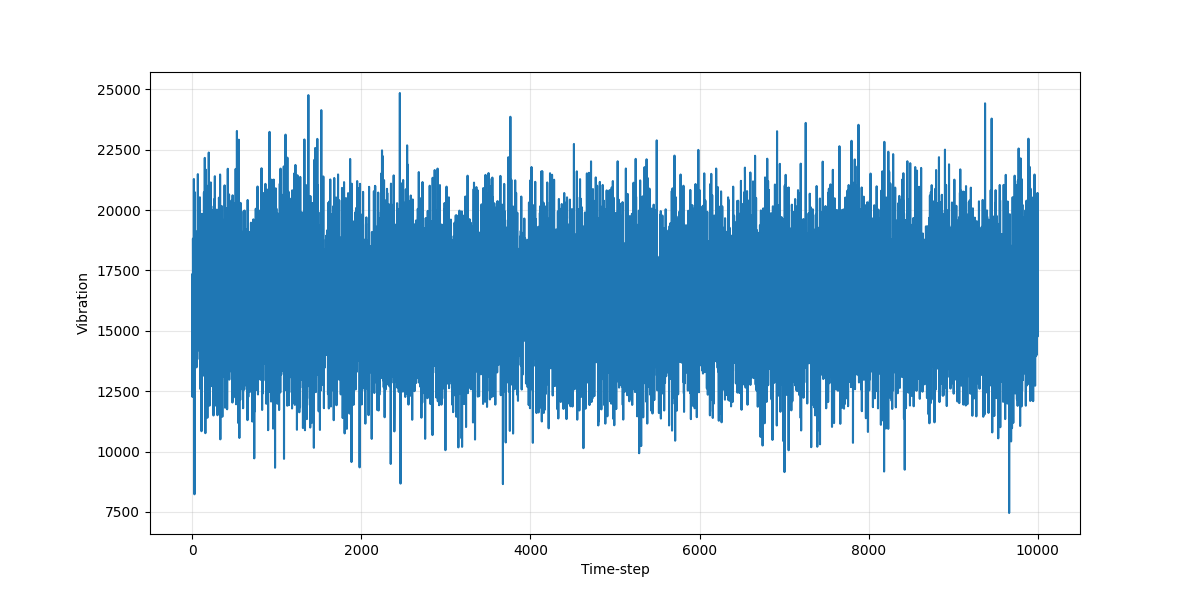
\includegraphics[width=0.7\textwidth]{figures/vibration_data.png}
\caption{Example of the raw vibration signal.}
\label{fig:BadExample}
\end{figure}
In contrast, transforming the data into a Time Delay Embedding phase space produces a highly compact visually informative fingerprint.Figure \ref{fig:tdeHealty} shows the baseline fingerprint under healthy normal operating conditions, generated with the algorithm described in Section \ref{section:OriginalImplementation} 
A healthy fingerprint is characterized by signal periodicity, which "results in elliptical structures and 'round' point cloud shapes" \cite{rakuschek2025visual}. Furthermore, "noise accumulates near the center while vibrations cause the circular patterns with a larger radius than noise," with these circular structures persisting even under high noise levels \cite{rakuschek2025visual}.
\begin{figure}[H]
\centering
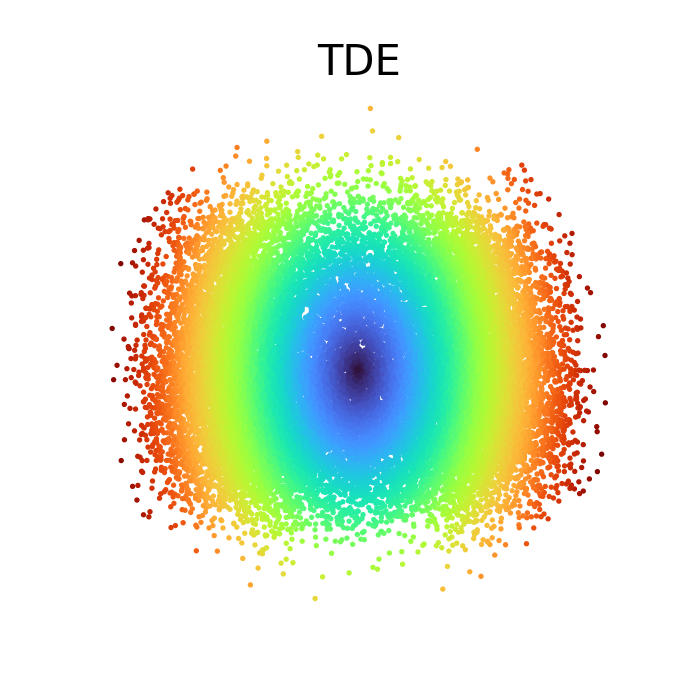
\includegraphics[width=0.5\textwidth]{figures/tdeVisual.png}
\caption{Example of a faulty fingerprint from a machine running in presence of mechanical imbalance at shaft.}
\label{fig:tdeBadExample}
\end{figure}
\begin{figure}[H]
\centering
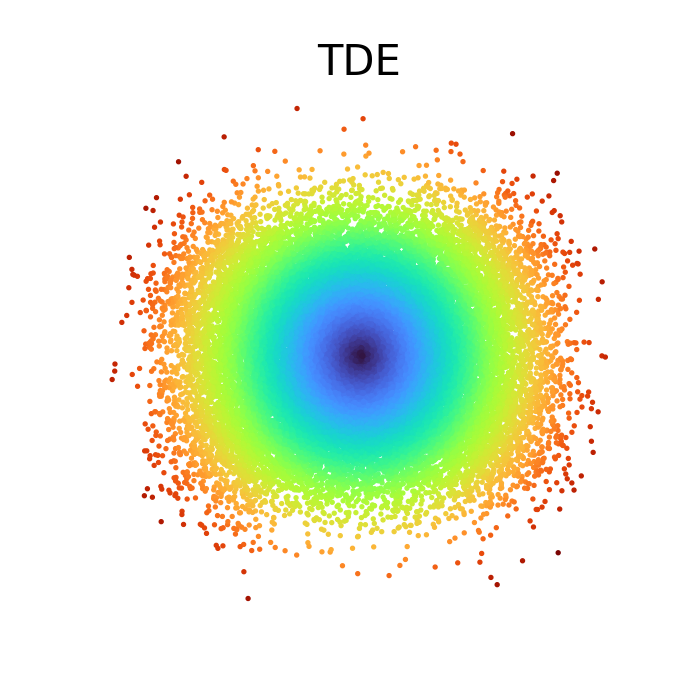
\includegraphics[width=0.5\textwidth]{figures/healtyFingerprint.png}
\caption{Example of a fingerprint under no faulty conditions.}
\label{fig:tdeHealty}
\end{figure}
Comparing the faulty fingerprint in Figure\ref{fig:tdeBadExample} with the healthy baseline in Figure \ref{fig:tdeHealty} shows distinct geometric distortions. For instance in figure \ref{fig:BadExample} a mechanical shaft imbalance wraps the phase trajectory into an asymmetric pattern while the healthy fingerprint shows a clean and periodic shape. 


\section{Related work}
\subsection{Incremental principal component analysis}
Conventional Principal component analysis requires storing all observations made over time and calculating full matrix eignedecomposition, introducing a high computational complexity which is unsuitable for real time anomaly detection. A smart solution is to shift the computational load to functions which are able to reuse already calculated values for its computation lowering the computational cost massively.Following the incremental principal component analysis framework introduced by \textcite{Incremental_PCA}, the proposed pipeline maintains running data statistics and updates the dominant eigenspace iteratively upon receiving each new observation.
Even with this optimization steps a central challenge remains: extracting the eigenvectors of the covariance matrix at every iteration step.  
According to \textcite[p.~2931]{1468483}, note that traditional signal subspace estimation relies on eigenvalue or singular value decomposition, whose inherent computational complexity creates a genuine need for fast subspace tracking techniques in adaptive signal processing. This motivates the subspace tracking approach, which instead avoids full eignedecomposition by iteratively refining an estimate of the dominant eigenvectors.
\subsection{Subspace tracking}
One problem that arises when working with principal component analysis is that the result, which is an covariance matrix, is often of higher dimension and computationally challenging to diagonalize directly via a full eignedecomposition. The subspace iteration method solves this issue by iteratively estimating the dominant eigenvectors instead of solving the eigenproblem at each iteration step. \textcite[p.~270]{Oja1982SimplifiedNM} proves that a simple Hebbian-type update rule combined with normalization converges with probability one to the dominant eigenvector of the input correlation matrix, provided the largest eigenvalue has multiplicity one. This provides the theoretical basis for implementing the subspace iteration method to solve the eigenvector problem.
Following this principle the eigenvector solver used in the principal component analysis routine follows the classical power iteration scheme described by \textcite[p.~2932]{1468483}, which alternates a data compression step—multiplying the correlation matrix by the current subspace estimate—with an orthonormalization step at each iteration.
However \textcite[p.~2932]{1468483} points out that the classical power iteration method is unsuitable for real-time processing due to its computational cost, which scales with the ambient dimension $n$ of the data; this motivated the development of faster approximations such as API and FAPI. 
To achieve fast convergence requires the covariance matrix to be kept as small as possible. Since in this thesis the covariance matrix is computed over the $d$-dimensional embedding space rather than on an large continuous array, the power iteration remains computationally stable for real time use without requiring these approximations.


\subsection{Phase Space Reconstruction and time delay embedding}
As summarized by \textcite{Tan_2023}, the embedding theorem guarantees that, 
\subsection{Sliding Window}
The sliding window approach is a method for processing steaming data using a fixed -size buffer that retains only the most recent observations. As new data arrives, older data points are discarded while more recent data points are continuously appended to the  buffer. \\ In the context of this thesis, the sliding window approach is applied to the time series data before the Time delay Embedding (Section 2.2.1) and Principal Component Analysis (Section 2.2.2). This fulfills the key requirement of handling steaming data efficiently while maintaining constant memory usage  and low latency.  \\
According (\cite{https://doi.org/10.1155/2014/879736} p.14 ), given a time series $T$ of length $m$ and a user-defined subsequence length $n$, all possible subsequences $C_p$ can be extracted by sliding a window of size $n$ across $T$.
This formalization reflects how sliding window mechanism extracts sequential segments from continuous time-series data.
\subsection{Industrial vibration monitoring solutions}
Two of the most established innovators in the field od real-time machine monitoring are Bently Nevada and Emerson, which offer a wide range of wireless and hardwired solutions along with corresponding data visualization. Their customers come from large-scale industries sectors such as power generation, mining and steel production. However the visualization provided typically remains limited to raw amplitude plots, which require high domain expertise and do not offer a an intuitive overview of machine health. 
\begin{figure}[H]
\centering
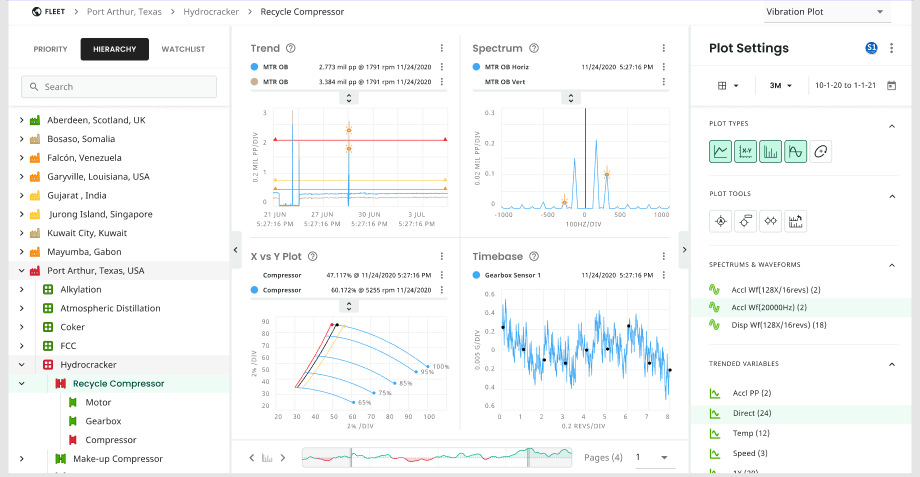
\includegraphics[width=0.8\textwidth]{figures/test2.png}
\caption{Dashboard example from a commercial condition-monitoring platform.\parencite{snyder2021roadmap}}
\label{fig:dashboardBentlyNevada}
\end{figure}
It must be pointed out that the data shown in figure \ref{fig:dashboardBentlyNevada} does not represent sensible customer data but rather only plots mock data for demonstration purposes provided by the vendor.
The dashboard provides an example offered by such platforms: \textcite{snyder2021roadmap} a full complement of diagnostic plots is provided, including polar, orbit, waveform, spectrum, waterfall, air gap, X-Y, multivariable trend, bode and amplitude phase time, and others. While this offers comprehensive coverage, no plot is designed ti make periodic behavior immediately visible at first sight. In contrast the system requires to interpret a specific aspect of the signal separately. A fingerprint plot such as the ones produced by principal component analysis would be a valuable extension to the already established workflows offering a better overview of periodicity and structural changes that normally would require cross referencing across multiple specialized plots.

% Checked with grammarly
\chapter{Methology}

% Checked with grammarly
\section{Used Programming language}
Since this thesis includes a actual implementation of the algorithm the decision of the tech stack is crucial for a successful project. One of the thesis requirements is the development of a cross-platform implementation. According to the specification, the implementation should be based on the procedural core of the C language family and should be usable across languages of the C family with only minimal modifications to the source code.
The procedural core means that the algorithmic core should be written in C, allowing it to be compiled using the GCC compiler. This core can then be easily integrated using lightweight wrappers in G++ or Java, while the computation itself remains entirely within the procedural layer.
% Checked with grammarly
\section{Tech stack}

For the development, Visual Studio Code was used due to the rich extensions marketplace and easy integration of C, C++ and Java programs (https://code.visualstudio.com/). Code formatting is handled by ClangFormat with a custom .clang-format configuration file to enforce an consistent style guide for improving readability and for maintaining a cleaner code base(https://clang.llvm.org/docs/ClangFormat.html).The main language which was used is C++17 and c11 due to the reasons explained in 3.1 Used Programming language.  For building and linking of the .cpp and .hpp source file the GNU C++ compiler (GCC 13.2.0) was used (https://gcc.gnu.org/). The build process is automated via a Makefile, which can be executed using \texttt{mingw32-make} on windows, \texttt{add here for linux} on Linux and \texttt{add here for mac} on Mac OS. Then to run the executable programm ./anomaly\_detection or just right away building and running by adding "run" to the make script shown before.
For the version control Git 2.53.0 is used and whole code is documented on GitHub with an clear introductions on how to use the code :\url{https://github.com/FabianSanterTUGraz/Real-time-Anomaly-Detection-in-Time-Series-Data}.While the \texttt{matplotlib.pyplot} library was utilized for initial data visualization, plotting functionality serves solely as a visual diagnostic tool for inspecting and comparing results, and is therefore excluded from the core algorithm specifications.
\section{Data validation}
The dataset used for validating the feasibility of the proposed approach and evaluating the overall functionality of the implementation is the \textit{Electric Motor Vibrations Dataset} provided by the SOON: Social Network of Machines CHIST-ERA Project (\cite{DATA_SET}). The dataset consists of 30 individual column separated values (CSV) files containing vibration measurements collected from two different electrical motors operating under different conditions. The appendix \ref{app:dataset_description} exactly documents each test condition in which the motors where tested in this thesis these different tests will be refereed by their individual ids.
Each dataset contains a timestamp value followed by acceleration measurements along the three spatial axes ($x$, $y$, and $z$). The timestamp column represents the time order of the measurements, while the remaining columns describe the recorded vibration signals of the sensor in the respective axes.
Before the data can be used for anomaly detection, two essential preprocessing and validation steps are required: First, the timestamps must be validated to ensure a consistent sampling interval across the dataset. Second, the three-dimensional acceleration vectors must be transformed into a single representative signal for easier processing.
\subsection{Sampling Interval ($\Delta$t)}
Consistent sampling intervals are important factors in time series data. Large time jumps between consecutive individual measurements can introduce artificial anomalies. Therefore the dataset was validated by calculating the time differences between consecutive timestamps. 
The interval $\Delta t$ was calculated as : \\
\begin{center}
$\Delta t_n = t_n - t_{n-1}$ \\
\end{center}   
Where $\Delta t_n$ is the time  difference between the current  and previous measurement. 
With Python's NumPy min and max functions, the minimum and maximum $\Delta t$ were computed for each dataset. The complete evaluation results are detailed in \ref{app:appendix2}. Inspection identified anomalies characterized by unexpected negative or excessively large values. After excluding these specific files  
(Files: 05, 13, 14, and 16) and running again the algorithm, the resulting statistical values improved significantly, as show in \ref{table:statistics}.\\
\begin{table}[!h]
 \centering
 \begin{tabular}{|c|c|}
 \hline
 Total number of intervals & 2,975,473 \\ 
 \hline
 Mean $\Delta t$ & 1,906.94 $\mu$s \\ 
 \hline
 Standard deviation & 38.03 $\mu$s \\ 
 \hline
 Median & 1,912.0 $\mu$s \\
 \hline
 Minimum & 1,660.0 $\mu$s \\
 \hline
 Maximum & 2,032.0 $\mu$s \\
 \hline
 \end{tabular}
 \caption{Statistics of sampling intervals after filtering rounded to the second decimal}
 \label{table:statistics}
\end{table}
\\
By analyzing the results, a clear improvement can be observed, the difference between the minimum, maximum, and the global mean are very small. Additionally, the standard deviation has improved a lot, which indicates highly consistent sampling. These results imply that the dataset was successful cleaned and can be used for further benchmarking and testing.
\subsection{Combining vectors}
A method for combining three orthogonal acceleration vectors into a single composite measure is the vector magnitude approach, as it preserves the total acceleration energy of the signal. By only taking the sum or average of the three axes bias might be introduced or important information might be lost. To obtain a single measure of total acceleration, the vector magnitude is calculated for each dataset using the theorem:
\begin{equation}
    VM = \sqrt{(x^2 + y^2 + z^2)}
\end{equation}
This method is supported by \cite{formulaCombiningVectors}, who state that "the VM equation is the square root of the sum of the squares of three planes of motion."
\chapter{Implementation}

\section{Architecture}
\subsection{Streaming Data}
The main data source are single column comma separated values files which are read by a stream of c++ library "fstreams". The stream is an independent object which is created in the main file with a corresponding file path. \\ \\
\lstinputlisting[
  language=C,
  caption={Object which handles the streaming of data.},
  label={src:linregressionalgorithm},
  firstnumber=1,
  firstline=1,
  lastline=36
]{content/codebase/streamingData.hpp}
Rather than loading complete dataset batches into memory, incoming sensor data is  processed line per line.
Data ingestion is encapsulated within a custom stream handler class (\texttt{streamData}), which wraps standard C++ file input streams (\texttt{std::ifstream}). The boolean flag (\texttt{bool next}) and (\texttt{bool hasNext}) are used to check if there are still some values left in the file which can be read by the handler.
To eliminate potential data crashes, data races and runtime memory reallocation overhead, all operational state buffers are pre-allocated on the stack during configuration.
Finally, the resulting principal component scores are accumulated in a dynamic buffer and written to disk (\texttt{output.txt}) upon successful completion of the algorithm execution.
\subsection{Sliding window with streaming data}
To process continuous time-series streams in real time, a sliding window of fixed capacity $N_{\text{window}}$ is maintained in memory. As the data stream yields new scalar values, the sliding window buffer is updated incrementally.\\ \\
During each iteration of the main loop, the window state is shifted left by one position via \texttt{slideWindow()}, forgetting the oldest sample at index 0 and appending the newest stream value to the terminal index $N_{\text{window}} - 1$. Adjusting the window size parameter directly controls the historical sample memory, allowing straightforward evaluation of parameter sensitivity on time-delay embedding (TDE) and covariance stability.
\subsection{Matrices and Vectors}
Do to the constrain that the implementation should be able to be used in all c-family with minimal changes the source code build in vectors should not be used. 
Instead, multidimensional matrices and state vectors are represented as contiguous 1D flat arrays. This design ensures consistent memory layouts across execution environments while simplifying low-level pointer arithmetic and dynamic memory management in C11.
\subsection{Time delay embedding}
It is the technique for reconstructing the underlying dynamics of the time series by transforming a signal into a higher order dimensional state space representation. The time delay embedding vector is defined as: 
\begin{equation}
\mathbf{z}_t = \begin{bmatrix}
x_t \\
x_{t-\tau} \\
x_{t-2\tau} \\
\vdots \\
x_{t-(d-1)\tau}
\end{bmatrix} 
\label{eq:tde_definition}
\end{equation}
In a sliding window implantation of length $W$(the buffer window size),the time-delay embedding vector $x_t \in R^d$ of dimension $d$ is extracted from the last element of the current window. Because the index offsets defining each embedding dimensions remain constant across iterations, they can be pre-calculated during initialization according to:
\begin{equation}
\text{index}_i = (W - 1) - i \cdot \tau, \quad i = 0, 1, \ldots, d-1
\label{eq:tde_indices}
\end{equation}
The values from the sliding window into the time delay embedding vector get mapped with this $index_i$ mapping. 





\subsection{Main program routine}
The main programm routine consits of a while loop which checks each iteration if there are still values to read in from the corresponding csv file until end of file (EOF) is reached. 


\section{Incremental PCA approach}
\subsection{Operations}
To ensure real-time responsiveness in principle component analysis each sub-step in the algorithm must work incrementally rather than recalculate values.
These operations to optimize are: running mean and covariance matrix, centering incoming vectors and updating feature directions.
\input{content/chapter4/incrementalPca/operations/mean}
\input{content/chapter4/incrementalPca/operations/covarianceMatrix}
\input{content/chapter4/incrementalPca/operations/subspaceIteration}



\section{Sliding Window Implementation}
\subsection{Data structure}
The sliding window is implemented as a fixed-size array, where the buffer size $w$ can be modified. The window is initialized by a dedicated function which reads the values from the specified comma separated values with the streaming approach explained in \ref{section:SlidingWindowWithStreamingData}. The resulting array is owned by the main function and can easily be passed to the the time delay embedding function for further operations. A main limitation is the update overhead: shifting the window requires $\mathcal{O}(w + s)$ time, where $w$ is the window size and $s$ the slide step.
\subsection{Visual explanation}
The sliding window mechanism maintains a buffer buffer of a fixed length over the most recent observations from the data stream. As new data arrives, the window advances(slides) forward by a defined step size, discarding older observations while keeping elements that overlap with the previous window. The result is a data structure which allows real-time processing of continuous streams while keeping memory usage constant.\\
Figure~\ref{fig:sliding-window} shows this concept using an input consisting of the values 1 to 9, a window size of 5, and a slide step of 2. In the first iteration $n=1$, the window contains the elements ([1,2,3,4,5]). Advancing by two positions produces, the next second window ([3,4,5,6,7]). A final shift produces the third window $n=3$([5,6,7,8,9]).\\
At the implentation level the \texttt{SlidingWindow::slideWindow()} function updates the window by removing the oldest \texttt{slideStep} elements and shifting the remaining elements to the left. The positions at the end of the window are then populated with new values from the input stream.

\begin{figure}[htbp]
    \centering
    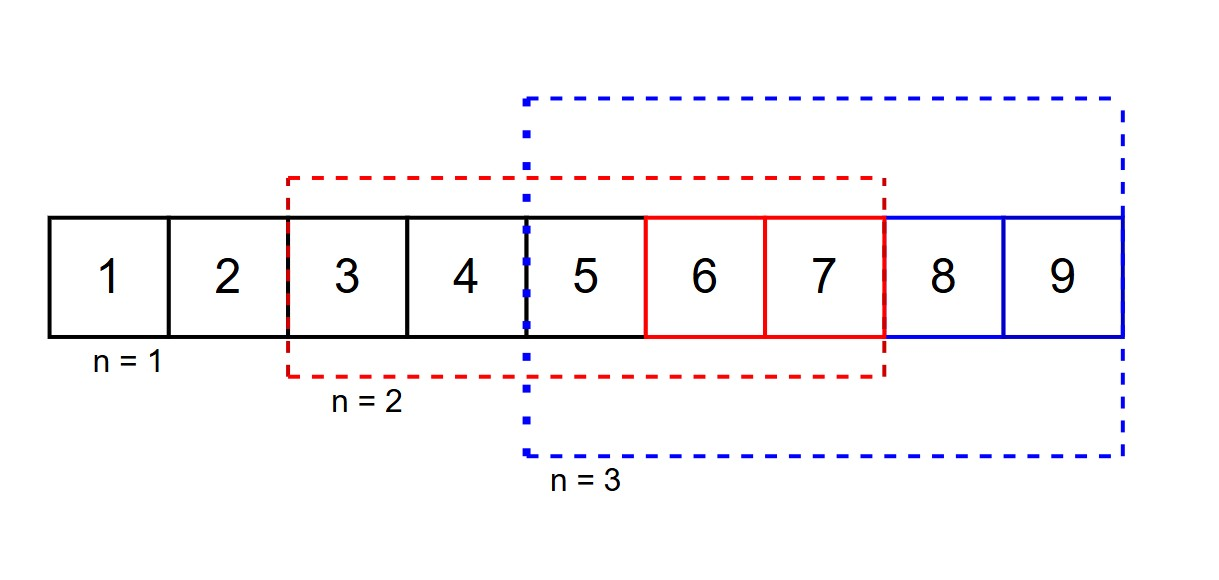
\includegraphics[width=0.35\textwidth]{figures/slidingWindowRepresentation.jpg}
    \caption{Example of a sliding window with n being the the iteration number.}
    \label{fig:sliding-window}
\end{figure}
\section{Integration time delay embedding vectors}
To reduce runtime computational overhead, the indexes offsets required for time-delay embeddings are precomputed once during initialization instead recalculating them from scratch at each streaming step. The embeddingIndexes function calculates these index positions based on the specified embedding dimensions and time lag parameter tau. 
\lstinputlisting[
  language=C,
  caption={All variables needed to call the algorythm},
  label={src:linregressionalgorithm},
  firstnumber=30,
  firstline=30,
  lastline=38
]{content/codebase/AnomalyDetection.c}
These index mappings remain constant trough execution and they are reused across all following iterations. Using these precomputed indexes, the embedding function extracts the corresponding values directly from the sliding window buffer to construct the current embedding vector.
\lstinputlisting[
  language=C,
  caption={All variables needed to call the algorythm},
  label={src:linregressionalgorithm},
  firstnumber=40,
  firstline=40,
  lastline=47
]{content/codebase/AnomalyDetection.c}
To ensure valid array indexing the sliding window must be sufficiently larger than $(d - 1) * \tau + 1$, where d is the embedding dimension and $\tau$ the time lag.
\section{Code integration into any project}
Since this bachelor thesis includes the implementation of the incremental principal component analysis algorithm, easy integration into existing or new software projects as well as further development within the project is desired. Since no language specific libraries where used the code should be easily adaptable other programming languages with minimal changes. The following chapter gives a brief overview on how to use the codebase.
\subsection{Data Containers}
\label{section:dataContainers}
Unlike programming languages which use automatic garbage collection (such as Java), dynamic memory management in C/C++ requires allocation strategies to eliminate memory fragmentation and buffer overflows. In consequent primary data variables are pre-allocated to the functions stack before the main API calls.
\lstinputlisting[
  language=C,
  caption={All variables needed to call the algorythm},
  label={src:linregressionalgorithm},
  firstnumber=44,
  firstline=44,
  lastline=70
]{content/codebase/code/anomaly_detection.cpp}
The data types were intentionally cheosen to be generic across the entire project to make sure to support a straightforward cross-implementation.
To reuse the code these initialization steps can be integrated directly. Only the delay parameter tau and the window size has to be adapted following the recommendations analyzed in the evaluation section \ref{section:influenceOfParameters}.
 \subsection{Main API call call}
 To offer modular software integration, the complete time delay embedding, sliding window and component analysis pipeline is exposed through a single function. This function directly takes the data containers detailed in the section \ref{section:dataContainers} and operates on them.
 \lstinputlisting[
  language=C,
  caption={Primary API function for real-time streaming data processing},
  label={src:linregressionalgorithm},
  firstnumber=4,
  firstline=4,
  lastline=19
]{content/codebase/AnomalyDetection.c}
The routine updates the running covariance matrix,performs subspace iteration to extract the dominant eigenvectors, and maps the resulting vectors onto the computed subspace. The output points outX and outY represents the coordinates on the reduced two dimensional coordinates along the first and second principal axes.\\
The subspace iteration returns orthonormal unit eigenvectors with a length of one, because of that computing the inner product via a dot product calculates the exact scalar projection length of the high dimensional time delay embedding vector onto each principal component.

\subsection{Example Usage}
The algorithm can process arbitrary time series data points, provided incoming samples are passed continuously to the processNewDataPoints function. In the reference demonstration, the projected coordinates are appended to a dedicated output vector and then written to an text file, however the output stream can also be integrated directly into a real-time visualization interface such as OpenGL or other similar plotting libraries. 
\lstinputlisting[
  language=C,
  caption={Example usage of the algorythm with streaming data},
  label={src:linregressionalgorithm},
  firstnumber=72,
  firstline=72,
  lastline=88
]{content/codebase/code/anomaly_detection.cpp}
The pipeline can process multiple concurrent data streams or also pause and resume execution. As a result
the underlying data sources and data storage remains decoupled from the core routine.
\subsection{Licensing}
Selecting an appropriate license is a critical final step in the software releasing process as it establishes the legal framework governing the access, modification, redistribution and commercial use of the codebase. Do to the fact that the thesis is of academic nature and tires to achieve maximum accessibility and promoting of collaboration, the source code is released under the MIT license. The MIT license offers minimal restrictions and straightforward terms. It grants users rights to reuse, copy, modify, merge, publish, distribute, sub-license and sell copies of the software. Furthermore, it includes a disclaimer of warranty and liability, thereby protecting the author from legal claims or damages resulting from use or execution of the code. The full license text can be found in appendix \ref{app:Licensing}.  
\section{Summary}
Chapter 4 Summary

\chapter{Evaluation and Validation}
\subsection{Visual comparison}
\label{section:VisualComparison}
To decide if the results of the streaming implementation and the offline approach by \textcite{rakuschek2025visual} match they are are visually compared. To compare them one to one the window size $W$ is set to span the entire length of the input sequence. Normally streaming operations use smaller windows which discard historical observations to adapt to non stationary dynamics, nevertheless this causes the covariance matrix to represent recent observations rather then the global sequence of distribution. Additionally the online subspace iterations requires an decent number of sample updates to converge to an stable solution. Short sequences would compare the offline baseline against an non converged subspace estimate.\\
The evaluation is done on the datasets No.2 and No.30 with their corresponding descriptions found in \ref{app:dataset_description}. The time delay embedding parameters are set to a time lag of $/\tau = 1$ and embedding dimension of $d=15$, matching the reference setup. To force asymptotic convergence of the subspace iteration toward the true principal axes the algorithm executes multiple times successively over the input dataset.
\begin{figure}[H]
\centering
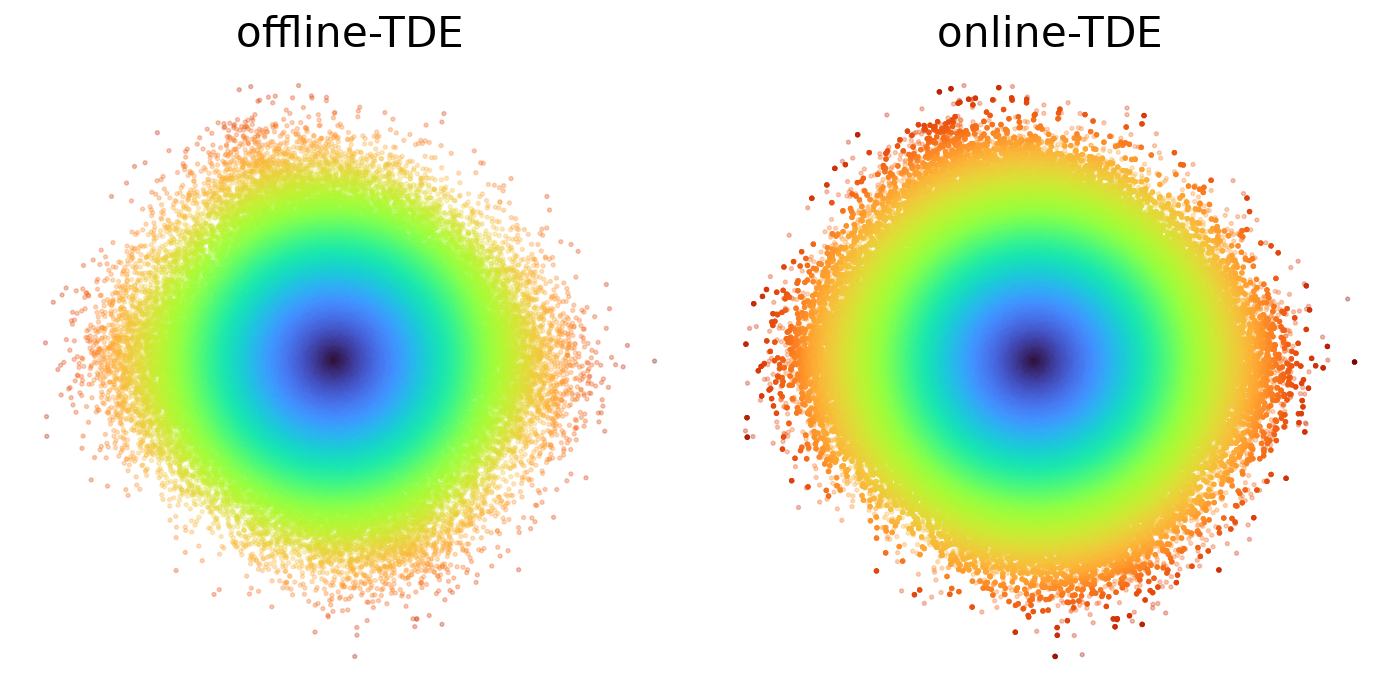
\includegraphics[width=1\textwidth]{figures/comparison_output_dataset2_d15_tau1_w102909.png}
\caption{Principle component analysis applied on dataset 02,with 102909 data points.}
\label{fig:tdeVisualComparison02}
\end{figure}
The plot generated from dataset 02 in figure \ref{fig:tdeVisualComparison02}(electric motor operating under healthy load and conditions) does not produce a distinct periodic shape in the projected subspace. The low amplitude vibrations characteristics of the normal operation  gather near the origin rather than forming a structured phase space geometry.
\begin{figure}[H]
\centering
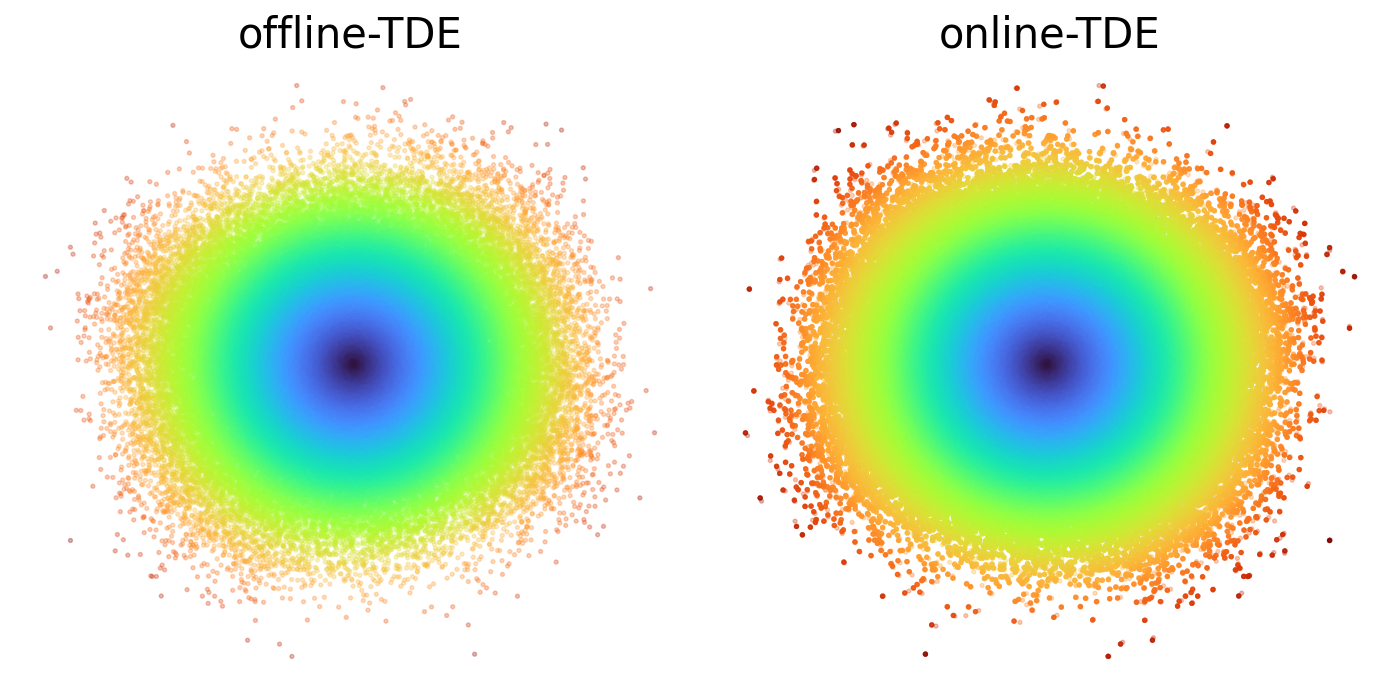
\includegraphics[width=1\textwidth]{figures/comparison_output_dataset30_d15_tau1_w101407.png}
\caption{Principle component analysis applied on dataset 30,with 102909 data points.}
\label{fig:tdeVisualComparison30}
\end{figure}
The comparison between the offline and online versions verifies that the streaming time delay embedding with principal component analysis and sliding windows produces correct values and generating visually identical structures.\\
Moreover this visual comparison produces an important insight regarding directly comparing "healthy" and "faulty" directly. Healthy states do not inherently produce clean  ellipsoid or ring like forms. As shown in Figure \ref{fig:tdeVisualComparison30},dataset 30(which contains mechanical faults with shaft misalignment) produces a significantly clearer continuous ring structure than the normal running condition Figure\ref{fig:tdeVisualComparison02}. This result emerges because high amplitude fault dynamics introduce strong harmonic components that forces the trajectory into phase space loops. This means diagnostic fingerprints cannot be evaluated by comparing an healthy and an faulty fingerprint next to each other. One solution would be to observe the phase space change over time which will be addresses in Section \ref{section:plotOverTime}
\subsection{Benchmarking against Reference Data}
\label{section:Against reference data}
To validate the implementation the tutorial by \cite{CheckForCorectness} is used as a reference, as it provides a full computation of an principal component analysis based on a small, deterministic dataset with 10 entries. The output of the incremental principal component analysis is compared step by step against the values reported in this reference. The sliding window is configured to span the entire input dataset $w = 10$ and the embedding dimension is set to $d =2$ corresponding to the two-dimensional input data additionally the time delay is set to $\tau = 0$ since the reference example does not involve any temporal lag.
\begin{figure}[htbp]
  \centering
  \setlength{\arraycolsep}{8pt}
  $\text{Data} = 
  \begin{array}{r|r}
    x & y \\
    \hline
    2.5 & 2.4 \\
    0.5 & 0.7 \\
    2.2 & 2.9 \\
    1.9 & 2.2 \\
    3.1 & 3.0 \\
    2.3 & 2.7 \\
    2.0 & 1.6 \\
    1.0 & 1.1 \\
    1.5 & 1.6 \\
    1.1 & 0.9
  \end{array}
  \qquad\qquad
  \text{DataAdjust} = 
  \begin{array}{r|r}
    x & y \\
    \hline
    .69 & .49 \\
    -1.31 & -1.21 \\
    .39 & .99 \\
    .09 & .29 \\
    1.29 & 1.09 \\
    .49 & .79 \\
    .19 & -.31 \\
    -.81 & -.81 \\
    -.31 & -.31 \\
    -.71 & -1.01
  \end{array}$
  \vspace{0.4cm}
  \caption{Reference dataset: original values (left) and mean-adjusted values (right).}
  \label{fig:pca_example_data}
\end{figure}
Due to the reason that the reference tutorial doesn't use time delay embedding or a sliding window approach, a alternative comparison setup is established for validation purposes. The setup executes a direct, one to one comparison between the individual stages of the implementation and the reference calculation. As a first step the data is centered and the mean is updated accordingly. This produces values that match the reference with only small deviations in the resulting covariance matrix. 
\begin{table}[htbp]
\centering
\begin{tabular}{lrrr}
\toprule
Quantity & Reference & Own Implementation & Absolute Difference \\
\midrule
Mean $x$          & 1.81         & 1.81      & $0$ \\
Mean $y$          & 1.91         & 1.91      & $0$ \\
$C_{11}$          & 0.616555556  & 0.616556  & $4.44 \times 10^{-7}$ \\
$C_{12} = C_{21}$ & 0.615444444  & 0.615444  & $4.44 \times 10^{-7}$ \\
$C_{22}$          & 0.716555556  & 0.716555  & $5.56 \times 10^{-7}$ \\
\bottomrule
\end{tabular}
\caption{Comparison of the mean vector and covariance matrix computed by the proposed implementation against the reference values.}
\label{tab:mean_cov_comparison}
\end{table}
In contrast to the reference tutorial, which calculates the eignedecomposition of the covariance matrix directly, the implementation extracts the the two principal components with subspace iteration, which is an iterative method that converges to the true eigenvector after some number of iteration. Since the used dataset is too small to trigger converging, the subspace iteration is executed repeatedly on the same covariance matrix until the resulting eigenvectors stabilize. A single iteration step per incoming samples as in the actual streaming data use case would produce extremely high deltas in the output. When the subspace iteration stabilizes after 200 iterations the resulting deltas are:  
\begin{table}[htbp]
\centering
\begin{tabular}{lrrr}
\toprule
Quantity & Reference & Own Implementation (sign-corrected) & Absolute Difference \\
\midrule
$u_{1,x}$ & 0.735178656  & 0.735179  & $3.44 \times 10^{-7}$ \\
$u_{1,y}$ & 0.677873399  & 0.677873  & $3.99 \times 10^{-7}$ \\
$u_{2,x}$ & 0.677873399  & 0.677873  & $3.99 \times 10^{-7}$ \\
$u_{2,y}$ & -0.735178656 & -0.735179 & $3.44 \times 10^{-7}$ \\
\bottomrule
\end{tabular}
\caption{Comparison of the converged principal components (eigenvectors), sign-corrected due to the inherent sign ambiguity of eigenvectors.}
\label{tab:eigenvector_comparison}
\end{table}
Finally, the mean adjusted data is projected onto the converged principal component with the largest eigenvalue. When comparing the results from the tutorial to the implementation the following are the results. 
\begin{table}[htbp]
\centering
\begin{tabular}{rrrr}
\toprule
Reference $x$ / $y$ & Own Implementation $x$ / $y$ & Abs. Diff. $x$ & Abs. Diff. $y$ \\
\midrule
-0.827970186 / -0.175115307 & -0.827970 / -0.175115 & $2.0 \times 10^{-7}$ & $1.4 \times 10^{-7}$ \\
 1.777580330 /  0.142857227 &  1.777580 /  0.142857 & $3.3 \times 10^{-7}$ & $2.3 \times 10^{-7}$ \\
-0.992197494 /  0.384374989 & -0.992198 /  0.384375 & $5.1 \times 10^{-7}$ & $1.1 \times 10^{-7}$ \\
-0.274210416 /  0.130417207 & -0.274211 /  0.130417 & $5.8 \times 10^{-7}$ & $2.1 \times 10^{-7}$ \\
-1.675801420 / -0.209498461 & -1.675800 / -0.209498 & $1.4 \times 10^{-6}$ & $4.6 \times 10^{-7}$ \\
-0.912949103 /  0.175282444 & -0.912949 /  0.175283 & $1.0 \times 10^{-7}$ & $5.6 \times 10^{-7}$ \\
 0.099109438 / -0.349824698 &  0.099109 / -0.349825 & $1.4 \times 10^{-7}$ & $3.0 \times 10^{-7}$ \\
 1.144572160 /  0.046417258 &  1.144570 /  0.046417 & $1.6 \times 10^{-6}$ & $1.4 \times 10^{-7}$ \\
 0.438046137 /  0.017764630 &  0.438046 /  0.017765 & $1.4 \times 10^{-7}$ & $7.0 \times 10^{-8}$ \\
 1.223820560 / -0.162675287 &  1.223820 / -0.162675 & $5.6 \times 10^{-7}$ & $2.9 \times 10^{-7}$ \\
\bottomrule
\end{tabular}
\caption{Comparison of the projected principal component scores between the reference and the proposed implementation, sign-corrected due to the inherent sign ambiguity of the underlying eigenvectors.}
\label{tab:scores_comparison}
\end{table}

// dazu schreiben ,dass man im grunde keine genaueren werte mit longs bekommen kann zwischen 10 hoch -5 und 10hoch -9 ist aktzeptabel
//vis datensätzte und https://github.com/OliverHennhoefer/awesome-ts-anomaly-detection-datasets

\subsection{Influence of parameter choices on the resulting fingerprint}
\label{section:influenceOfParameters}
The choice of parameters is a crucial decision for the quality of the resulting fingerprint plot. The main parameters which influence the outcome are window size $w$, the time delay tau $\tau$ and the embedding dimension $d$. The goal is to find out how these parameters influence the resulting visualization and to identify which settings produce plots with maximal information content and clear visual distinction between normal and distorted vibration patterns. 
\subsection{Plottin over time}
\label{section:plotOverTime}
As addressed in chapter \ref{section:VisualComparison} the one to one comparison between an healty and faulty fingerprint does not give a exact insight over the current status of the machine. Because of that plotting over time with the online principal component analysis is tested by keeping small windows and stop the routine and plot the result after n,n and n iteraations therby also proofing the incremental property of the algorythm.


 

\include{content/lessons_learned}
\include{content/conclusion}

\printbibliography              %% remove, if using BibTeX instead of biblatex

\appendix                       %% closes main document, appendix follows
\addpart*{Appendix}             %% adding Appendix to tableofcontents
\chapter{Dataset Description}
\label{app:dataset_description}
\section{Appendix 1}
\label{app:descriptionDataset}
\centering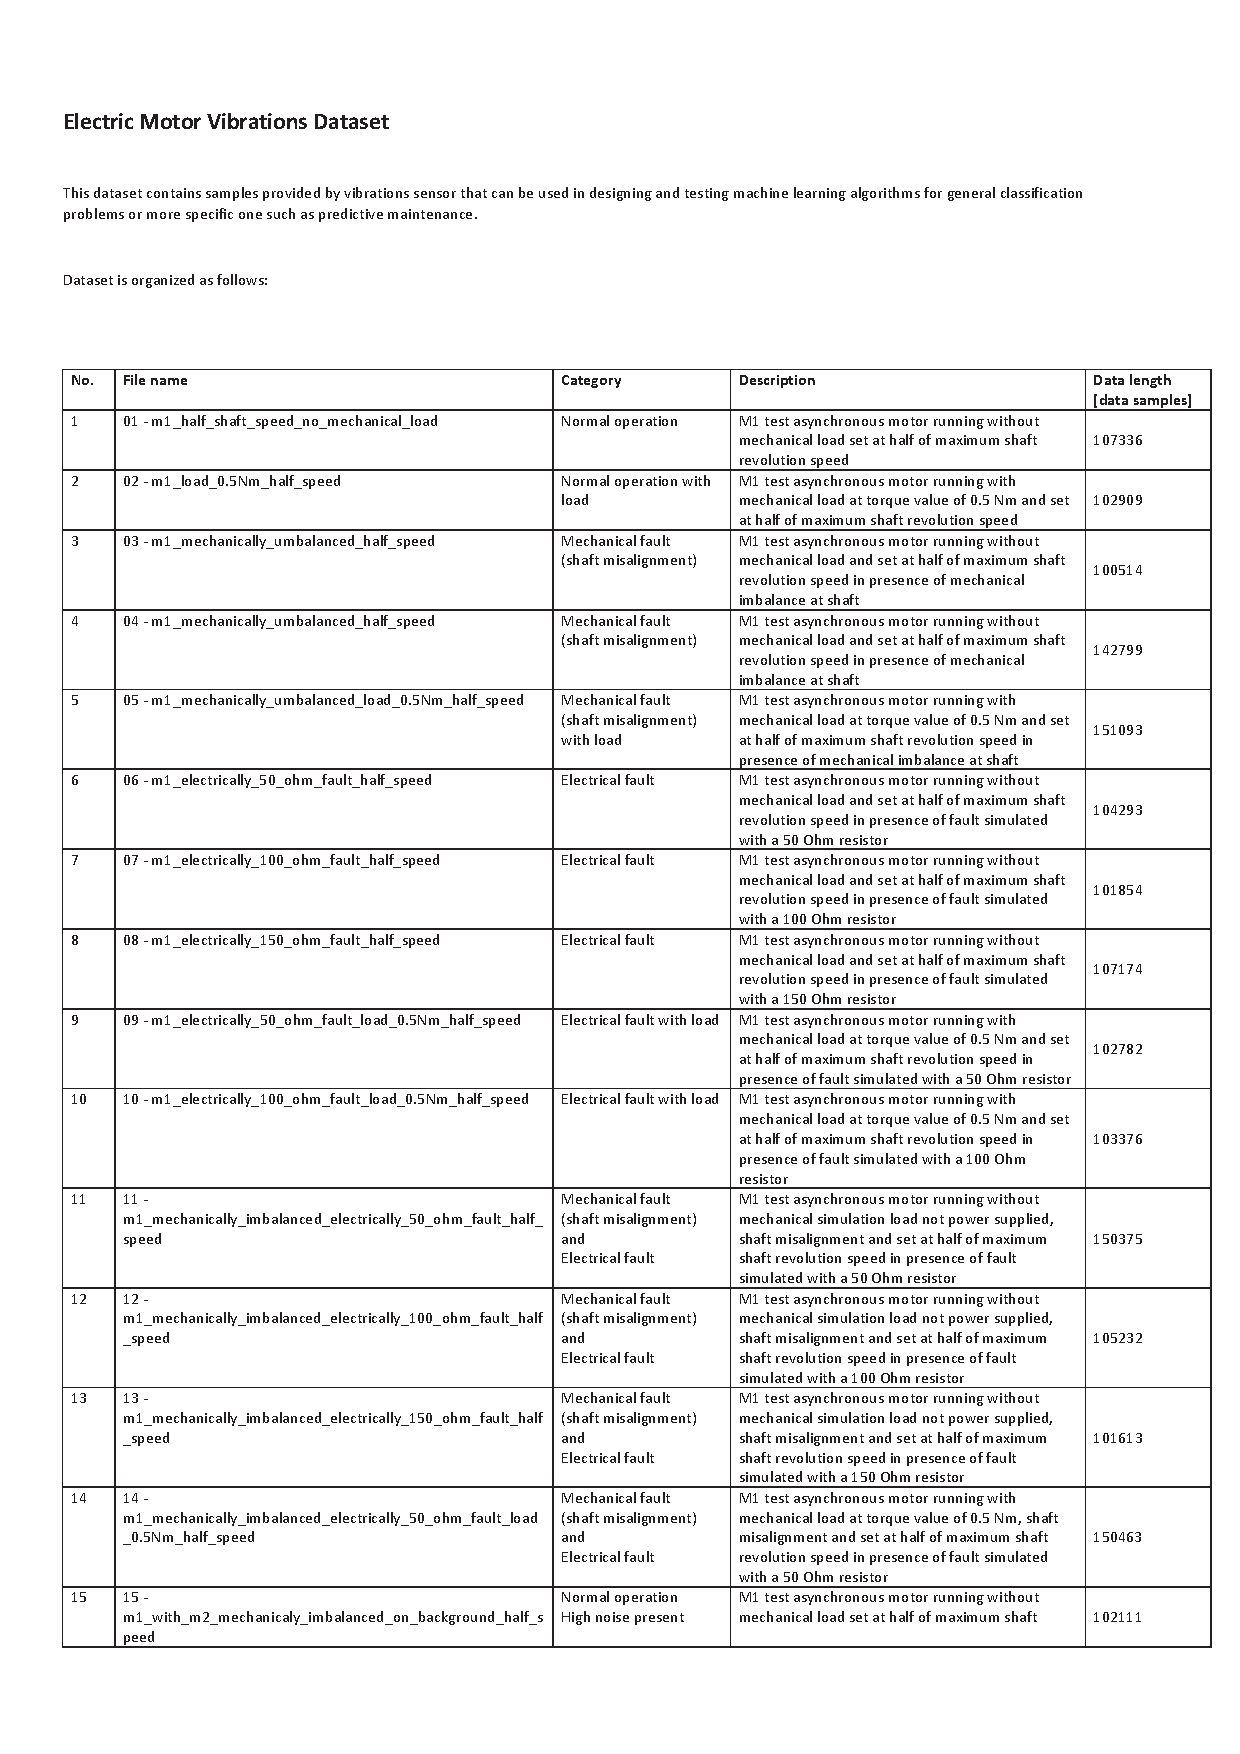
\includegraphics[page = 1, width=\textwidth]{content/appendix/Description.pdf}
\centering\includegraphics[page = 2, width=\textwidth]{content/appendix/Description.pdf}
\centering\includegraphics[page = 3, width=\textwidth]{content/appendix/Description.pdf}



\chapter{Per-File Sampling Interval Statistics}
\label{app:delta_statistics}
\section{Resulting statistics}
\label{app:appendix2}
\verbatiminput{content/appendix/results.txt}

\chapter{Codebase}
\label{app:excluded_files}
\section{Original implementation}
\lstinputlisting[
  language=Python]
{content/codebase/benchmarkCode/static_fingerprintvisualization.py}

\section{Main algorithm logic}
\lstinputlisting[
  language=C]
{content/codebase/code/include/AnomalyDetection.h}
\lstinputlisting[
  language=C]
{content/codebase/code/src/AnomalyDetection.c}

\section{Function calling}
\lstinputlisting[
  language=C]
{content/codebase/code/anomaly_detection.cpp}

\section{Plotting}
\lstinputlisting[
  language=Python]
{content/codebase/code/plotting.py}





\input{content/appendix/MIT}

\end{document}